\documentclass[11pt,a4paper]{article}
\usepackage[T1]{fontenc}
\usepackage[utf8]{inputenc}
\usepackage{lmodern}
\usepackage[margin=25mm]{geometry}
\usepackage{amsmath,amssymb,booktabs}
\usepackage{graphicx}
\usepackage[hidelinks]{hyperref}
\hypersetup{pdftitle={Optimizing N-Body Simulation: OpenMP baseline},
            pdfauthor={Semester project in parallel programming}}
\setlength{\parindent}{0pt}
\setlength{\parskip}{6pt}
\title{Optimizing N-Body Simulation\\\large Correctness, strong scaling and the first OpenMP profile}
\author{Semester project in parallel programming}
\date{17 November 2026}

\begin{document}
\maketitle

\section{Objective and current scope}
The project studies a direct three-dimensional gravitational simulation in
C++20 and OpenMP. This report records a sequential solver, a baseline parallel
solver, their shared Velocity Verlet integrator, and independent correctness
checks. A first experiment measures strong scaling on two fixed problem sizes.
A Windows sampling profile locates the code executed by the OpenMP workers.
The implementation uses double precision and provisional educational data.

The final report will target 12--18 pages of main text. Definitive input data,
convergence, selection and testing of an optimization, and visualization remain
future work. The learner's guided analysis of the code and profile is pending.

\section{State and softened gravitational model}
Each body has a positive mass $m_i$, a position $\mathbf r_i$, and a velocity
$\mathbf v_i$. Bodies are stored in a contiguous \texttt{std::vector<Body>}.
Current and next accelerations are stored in two separate vectors of
\texttt{Vec3}; there is no interaction matrix.

For source $j$ and target $i$, define
\begin{align}
 \mathbf d_{ij} &= \mathbf r_j-\mathbf r_i,\\
 q_{ij} &= \mathbf d_{ij}\cdot\mathbf d_{ij}+\epsilon^2,\\
 \mathbf a_i &= \sum_{\substack{j=0\\j\ne i}}^{N-1}
       \mathbf d_{ij}\frac{Gm_j}{q_{ij}\sqrt{q_{ij}}}.
\end{align}
Here $G>0$ and $\epsilon>0$. The target mass is absent from its acceleration.
Positive softening removes the zero-distance denominator for moderate inputs.
All source positions and masses remain unchanged during a complete force
evaluation. The sequential and parallel solvers use the same source order.

\section{Velocity Verlet and phase dependencies}
Compute $\mathbf a^0$ from the initial positions before entering the time loop.
For a fixed step $\Delta t>0$, execute
\begin{align}
 \mathbf r_i^{n+1} &= \mathbf r_i^n + \mathbf v_i^n\Delta t
                  + \tfrac12\mathbf a_i^n\Delta t^2,\\
 \mathbf a^{n+1} &= A(\mathbf r^{n+1}),\\
 \mathbf v_i^{n+1} &= \mathbf v_i^n
                  + \tfrac12(\mathbf a_i^n+\mathbf a_i^{n+1})\Delta t.
\end{align}
Every position update must finish before $A$ reads the new state. All new
accelerations must be available before the velocity update. Finally, swap
the two acceleration buffers. This reuses $\mathbf a^{n+1}$ at the next step.
One integrator selects the solver through a simple enum. The time loop and
both state-update loops remain sequential.

\section{Computational work and storage}
One full evaluation contains $N(N-1)$ directed pair contributions.
For $K$ steps, initialization plus one evaluation per step gives exactly
$K+1$ evaluations and $(K+1)N(N-1)$ contributions. Validation and state
updates add linear passes. Force work is quadratic in $N$; parallel execution
does not change that algorithmic complexity.

Bodies and two acceleration buffers require $\Theta(N)$ storage. No complete
trajectory is retained. Storing all $K+1$ states in a later export feature
would instead require $\Theta((K+1)N)$ storage. This cost is not incurred by
the current integrator.

\section{OpenMP decomposition and memory safety}
Only the outer loop over targets is parallel:
\begin{verbatim}
#pragma omp parallel for default(none) schedule(static) \
    shared(bodies, parameters, accelerations, observed_thread_count) \
    firstprivate(body_count)
\end{verbatim}
The acceleration output is allocated before the region. Each iteration owns
one target, accumulates in a local vector, and writes only its own output
element. Bodies and physical parameters are shared read-only. The inner
source loop is sequential. No global reduction, lock, or atomic is required.

The implicit barrier at the end of the region completes all outputs before
they are checked or consumed. An optional diagnostic, disabled by default,
records \texttt{omp\_get\_num\_threads()} only in target iteration zero. A
single writer and the final barrier make this diagnostic safe. It measures
the actual force-computation team, not a separate probe region.

\section{Inputs and numerical boundaries}
At solver entry, reject non-finite state, nonpositive masses, invalid $G$ or
$\epsilon$, and acceleration arrays whose size differs from the body count.
Simulation also requires a valid solver, positive finite $\Delta t$, and a
finite nonzero squared-step coefficient. Checks precede parallel work.
Non-finite force outputs are rejected after the region, without exceptions
escaping a worker.

Empty systems are valid and launch no parallel region. One isolated body has
zero acceleration and constant velocity. Zero steps evaluate the initial
accelerations but leave positions and velocities unchanged. Numerical failure
during in-place evolution does not roll back partial updates; discard that
result. Direct products in double precision do not provide general protection
against extreme scales or all underflow cases.

\section{Provisional examples}
Use normalized units $M$, $L$, $T$: velocities have units $L/T$, accelerations
$L/T^2$, and $G$ has units $L^3/(MT^2)$. Both examples set $G=1$; no SI or
astronomical interpretation is implied. The teacher's individual variant is
still unavailable.

\subsection{Two-body arithmetic reference}
Body A has $m_A=2$, $\mathbf r_A=(0,0,0)$; body B has $m_B=10$,
$\mathbf r_B=(0,3,0)$. Both velocities start at zero. Set $\epsilon=4$ to
obtain $q=25$ and $q\sqrt q=125$. Thus
\[
 \mathbf a_A=(0,0.24,0),\qquad \mathbf a_B=(0,-0.048,0).
\]
The opposing forces satisfy $m_A\mathbf a_A+m_B\mathbf a_B=\mathbf 0$.
This softening choice simplifies arithmetic; it is not a scientific
recommendation. The one-step integration reference uses $\Delta t=0.5$.

\subsection{Four-body deterministic example}
Use $\epsilon=0.1$ and the explicit initial state below. The demonstration
executes 25 steps at $\Delta t=0.01$. This case is not claimed to be in equilibrium.
\begin{center}
\small
\begin{tabular}{crrr}
\toprule
Body & Mass & Position & Velocity \\
\midrule
0 & 2 & $(-1,0,0.5)$ & $(0.05,0.10,-0.02)$ \\
1 & 1.5 & $(1,0.5,-0.5)$ & $(-0.10,0.02,0.03)$ \\
2 & 0.75 & $(0,-1,1)$ & $(0.04,-0.03,0.08)$ \\
3 & 3 & $(0.5,1.5,0.25)$ & $(-0.02,0.06,-0.04)$ \\
\bottomrule
\end{tabular}
\end{center}

\section{Validation actually performed}
Local builds used GCC 16.2.0 from MSYS2 UCRT64 with C++20 and OpenMP on
Windows 11, Intel Core 7 150U (10 physical cores, 12 logical processors).
Both existing CMake presets configured and compiled without compiler warnings.
CTest passed the six original tests in Debug and Release. The benchmark added
two integration checks covering solver equivalence and zero steps. All eight
entries then passed in each configuration.
Checks use explicit diagnostics and exit codes, so they remain active with
\texttt{NDEBUG}.

The independent reference literals for the two-body step are:
\begin{center}
\begin{tabular}{ll}
\toprule
Quantity & Expected $y$ component \\
\midrule
Position A & $0.03$ \\
Position B & $2.994$ \\
Velocity A & $0.12005194016285471$ \\
Velocity B & $-0.024010388032570942$ \\
\bottomrule
\end{tabular}
\end{center}
All other components are zero. Both solver modes passed these references.
For example, the printed Release velocities were
$0.12005194016285471$ and $-0.024010388032570943$ along $y$.
Expected values are not computed by the tested implementation.

Physics and equivalence comparisons reject non-finite values and require
\[
 |x-y|\leq 10^{-12}+10^{-12}\max(|x|,|y|).
\]
For both examples, accelerations and integrated states were compared at
0, 1, 2 and 25 steps with 1, 2 and 4 requested threads. Observed teams were
respectively 1, 2 and 4 in the actual force loop. Independent physics tests
are essential: agreement between solvers alone would also allow shared bugs.

Additional checks cover vector arithmetic, preserved inputs and masses,
opposite forces, isolated uniform motion, coincident bodies, empty systems,
zero steps, output sizes, invalid inputs and numeric failures. Ten continuous
steps match ten restarted one-step calls, checking acceleration reuse.
Fourteen CLI error cases require both the expected message and exit code 1.
Sequential and OpenMP demonstrations were run on both examples.

\section{First strong-scaling experiment}
The machine ran Windows 11 Home build 26300 on the Core 7 150U described
above. We used the Balanced power plan, UCRT64 GCC 16.2.0, libgomp and
the Release flags \texttt{-O3 -DNDEBUG -std=c++20 -fopenmp}, plus warnings.
The working tree contained local changes above commit \texttt{9bd8716}.
The binary, source fingerprints and effective commands are recorded in
\path{results/baseline/metadata.json}. Thread placement, background load
and CPU frequency were uncontrolled.

\textbf{Workload.} The generator uses the upper 53 bits of each draw from
\texttt{mt19937\_64} with seed 20261117. It draws a mass in $[0.5,1.5)$,
three position coordinates in $[-1,1)$ and three velocity coordinates in
$[-0.1,0.1)$ per body. We set $G=1$, $\epsilon=0.05$, $\Delta t=0.0005$
and $K=12$. A one-round pilot gave sequential times of 10.4, 98.9 and
486.7\,ms at 512, 1,536 and 3,072 bodies. The 12-thread times were 6.8,
42.1 and 131.6\,ms. The latter two sizes kept trials measurable at all
requested thread counts and affordable to repeat.

\textbf{Timing boundary.} Each configuration uses fresh copies of one master
state per size. A checked warm-up validates every final position and velocity
against the true sequential reference using the tolerance above and records
the actual team. The measured run starts its \texttt{steady\_clock} interval
at the initial force evaluation and stops after the last buffer swap. This
includes all 13 force evaluations and both linear state-update phases.
The per-pair numerical guard remains in the shared force code. Copies,
allocations, diagnostic scans, comparisons, fingerprints and file output are
outside the interval. The benchmark verifies each measured final state again.

\textbf{Order.} Each size ran six configurations for six rounds. Round one
started with sequential, followed by OpenMP 1, 2, 4, 8 and 12. The starting
configuration advanced one place per round. Each configuration occupied
each order position once. The two sizes ran consecutively. The controls
observed each requested team size in the actual target loop.

\clearpage
\section{Unprofiled Release results}
For each case, $S_p=\operatorname{median}(T_{\rm seq})/
\operatorname{median}(T_{{\rm omp},p})$ and $E_p=S_p/p$. The interquartile
range (IQR) is $Q_3-Q_1$ using inclusive linear interpolation. Each row
summarizes six simulations. The sequential rows define the reference.

\begin{center}
\small
\begin{tabular}{rlrrrrr}
\toprule
$N$ & Solver & $p$ & Median (ms) & IQR (ms) & $S_p$ & $E_p$ (\%) \\
\midrule
1,536 & Sequential & 1 & 115.6 & 7.4 & 1.00 & 100.0 \\
1,536 & OpenMP & 1 & 120.9 & 4.5 & 0.96 & 95.7 \\
1,536 & OpenMP & 2 & 68.2 & 5.2 & 1.70 & 84.8 \\
1,536 & OpenMP & 4 & 53.9 & 1.8 & 2.15 & 53.7 \\
1,536 & OpenMP & 8 & 43.6 & 2.3 & 2.65 & 33.1 \\
1,536 & OpenMP & 12 & 39.4 & 1.7 & 2.94 & 24.5 \\
\addlinespace
3,072 & Sequential & 1 & 479.7 & 9.3 & 1.00 & 100.0 \\
3,072 & OpenMP & 1 & 484.1 & 25.5 & 0.99 & 99.1 \\
3,072 & OpenMP & 2 & 265.8 & 25.1 & 1.80 & 90.2 \\
3,072 & OpenMP & 4 & 219.4 & 24.5 & 2.19 & 54.6 \\
3,072 & OpenMP & 8 & 164.8 & 8.4 & 2.91 & 36.4 \\
3,072 & OpenMP & 12 & 135.3 & 1.3 & 3.54 & 29.5 \\
\bottomrule
\end{tabular}

\end{center}

\begin{figure}[ht]
\centering
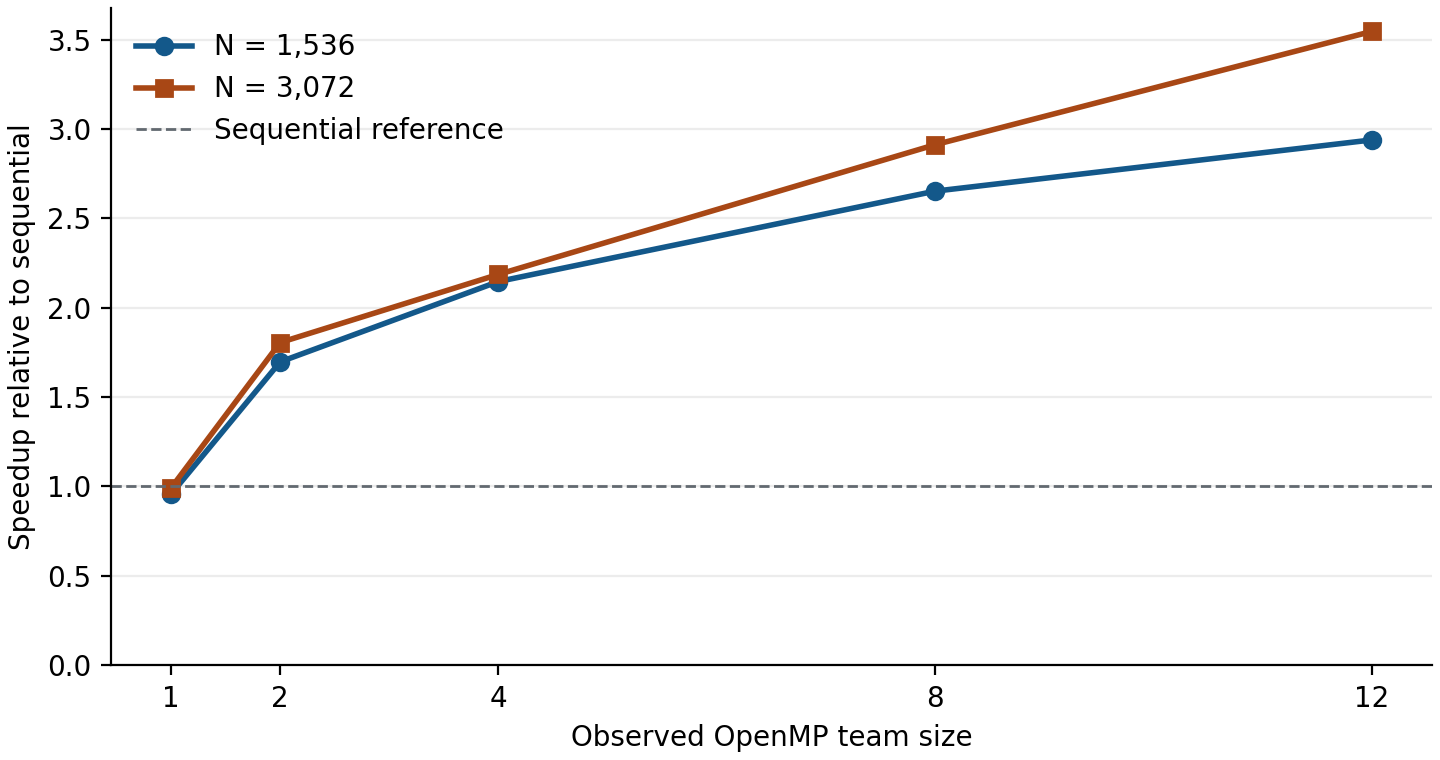
\includegraphics[width=0.90\linewidth]{results/baseline/speedup.png}
\caption{Strong scaling from 72 unprofiled runs. Each point uses the
sequential median at the same $N$. The dashed line marks unit speedup.}
\end{figure}

The serial and one-thread OpenMP medians differ by 5.2 and 4.4\,ms.
At $N=3{,}072$ the one-thread OpenMP IQR is 25.5\,ms, so these differences
do not isolate the cost of entering a parallel region. At 12 threads the
larger case reached $3.54\times$ speedup and 29.5\% efficiency. Increasing
$N$ doubled the number of targets and nearly quadrupled the directed
pair contributions, from 30,650,880 to 122,643,456 per run.

\clearpage
\section{Sampling the four-thread force loop}
We built a separate UCRT64 Release executable with the same compiler flags
and \texttt{-g}. It repeated the 3,072-body, 12-step, four-thread case
60 times from its original state. Every batch yielded the same final
fingerprint as the unprofiled campaign. The MSYS2 Cygwin
\href{https://cygwin.com/cygwin-ug-net/profiler.html}{sampling profiler}
(3.6.10) attached to the initialized Windows process at a requested
100\,Hz. The capture covered the remaining workload, including checks and
fingerprints between batches.

\textbf{Thread activity.} Windows reported individual thread events and
the loaded GNU OpenMP runtime. We also read OS user and kernel CPU counters
twice for the same process during sampling. In 3.432\,s of wall time, four
thread IDs accumulated 2.688, 2.453, 2.641 and 2.688 CPU seconds.
All seven threads present at both snapshots accumulated 10.484 CPU seconds
in total. Wall time advances once for the observer. CPU time adds the time
each thread actually executes, including overlapping execution.

\textbf{Function attribution.} The profiler periodically reads thread
instruction pointers, including those of threads in waits, and groups hits
by module. For the executable we translated the runtime addresses to the
linked \texttt{.text} section to account for Windows address randomization.
GNU \texttt{addr2line} then recovered the GCC inline chain at each four-byte
bin start. The archive includes the detached GCC symbols, the native
histogram and SHA-256 fingerprints of their inputs. The sample counts were:

\begin{center}
\small
\begin{tabular}{lr}
\toprule
Population & Sampled instruction pointers \\
\midrule
All mapped modules & 10,471 \\
\quad Windows \texttt{ntdll.dll} & 5,552 \\
\quad Other DLLs combined & 3 \\
\quad Benchmark executable & 4,916 \\
\qquad Of executable hits, in the OpenMP target loop & 4,914 \\
\bottomrule
\end{tabular}
\end{center}

The target loop accounts for 99.96\% of executable hits.
At linked bin \texttt{0x140002fd4}, 961 samples resolve to vector
multiplication in the inline chain through the gravitational contribution and
the per-target source loop. The sample bins pool threads. Their counts do
not measure elapsed seconds, useful CPU cycles or barrier waiting time.
Function attribution alone cannot tell whether arithmetic latency, memory
stalls or arrival imbalance explains the scaling curve.

\textbf{Evidence for the next experiment.} Divider-active cycles and
data-cache stall counters on a fixed core type could test an arithmetic
limit in the force loop. Per-worker arrival times at each force barrier
could test imbalance between workers. Selection of an optimization follows
those measurements and the learner's interpretation.

The raw CSV, complete final states, figure generator, profile exports and
exact reproduction commands are indexed in \path{docs/baseline-performance.md}.
Definitive assignment data, convergence and long-term invariant tests,
an optimized comparison and trajectory visualization remain future stages.

\end{document}
